\documentclass{article}\usepackage[]{graphicx}\usepackage[]{color}
%% maxwidth is the original width if it is less than linewidth
%% otherwise use linewidth (to make sure the graphics do not exceed the margin)
\makeatletter
\def\maxwidth{ %
  \ifdim\Gin@nat@width>\linewidth
    \linewidth
  \else
    \Gin@nat@width
  \fi
}
\makeatother

\definecolor{fgcolor}{rgb}{0.345, 0.345, 0.345}
\newcommand{\hlnum}[1]{\textcolor[rgb]{0.686,0.059,0.569}{#1}}%
\newcommand{\hlstr}[1]{\textcolor[rgb]{0.192,0.494,0.8}{#1}}%
\newcommand{\hlcom}[1]{\textcolor[rgb]{0.678,0.584,0.686}{\textit{#1}}}%
\newcommand{\hlopt}[1]{\textcolor[rgb]{0,0,0}{#1}}%
\newcommand{\hlstd}[1]{\textcolor[rgb]{0.345,0.345,0.345}{#1}}%
\newcommand{\hlkwa}[1]{\textcolor[rgb]{0.161,0.373,0.58}{\textbf{#1}}}%
\newcommand{\hlkwb}[1]{\textcolor[rgb]{0.69,0.353,0.396}{#1}}%
\newcommand{\hlkwc}[1]{\textcolor[rgb]{0.333,0.667,0.333}{#1}}%
\newcommand{\hlkwd}[1]{\textcolor[rgb]{0.737,0.353,0.396}{\textbf{#1}}}%
\let\hlipl\hlkwb

\usepackage{framed}
\makeatletter
\newenvironment{kframe}{%
 \def\at@end@of@kframe{}%
 \ifinner\ifhmode%
  \def\at@end@of@kframe{\end{minipage}}%
  \begin{minipage}{\columnwidth}%
 \fi\fi%
 \def\FrameCommand##1{\hskip\@totalleftmargin \hskip-\fboxsep
 \colorbox{shadecolor}{##1}\hskip-\fboxsep
     % There is no \\@totalrightmargin, so:
     \hskip-\linewidth \hskip-\@totalleftmargin \hskip\columnwidth}%
 \MakeFramed {\advance\hsize-\width
   \@totalleftmargin\z@ \linewidth\hsize
   \@setminipage}}%
 {\par\unskip\endMakeFramed%
 \at@end@of@kframe}
\makeatother

\definecolor{shadecolor}{rgb}{.97, .97, .97}
\definecolor{messagecolor}{rgb}{0, 0, 0}
\definecolor{warningcolor}{rgb}{1, 0, 1}
\definecolor{errorcolor}{rgb}{1, 0, 0}
\newenvironment{knitrout}{}{} % an empty environment to be redefined in TeX

\usepackage{alltt}
\usepackage{graphicx}
\graphicspath{{images/}}
\IfFileExists{upquote.sty}{\usepackage{upquote}}{}
\begin{document}

\textbf{Background: Footwear and Forensic Analysis}

In forensic science, shoe prints and outsole characteristics fall into the category of pattern evidence. When a shoe print is found at a crime scene, there are a number of questions that can be asked. For example, an investigator may want to determine the make or model of the show that made the print, or possibly tie the shoe print to a specific individual. Another question, more difficult than the first two, is how common the shoe type, or features of that shoe type, are in a local population. This question is more difficult than the first two because it relies not only on the information contained in the found print, but also on characteristics of many other types other shoes. Thus, any sufficient answer to this question requires a way to automatically and efficiently classify many different types of shoes within a common system.


\textbf{Classification}

Visual classification is a complex task that our brains have been trained to do very well. Our eyes detect a large variety of features of an object, including color, shape, and texture, and send that information to our brain. Our brain then learns which combinations of features to associate with a given label, and should be able to apply those rules to future objects with similar characteristics. For example, an orange caterpillar and a baby carrot may be of similar color, shape, and size, but one is distinctly more fuzzy than the other. Thus, our brains learn that when faced with a small, cylindrical orange object, texture becomes an important feature when assigning a label to that object (which keeps us from accidentally ingesting caterpillars). 

\textbf{Convolutional Neural Networks (CNNs)}

While our brains are adept at parsing images and classifying the objects within them, the task has proved much more difficult for computers. Convolutional neural networks (CNNs) are a tool for supervised deep-learning that have become standard in recent years for automatic image classification. CNNS use combinations of convolutional and pooling hidden layers to filter raw information into features, which are then fed into densely connected layers which are trained to associate given sets of features with their desired labels. This translation-invariant automated classification mimics the human eye-to-brain classification process and has become one of the most widely used machine learning techniques for image classification.


\centerline{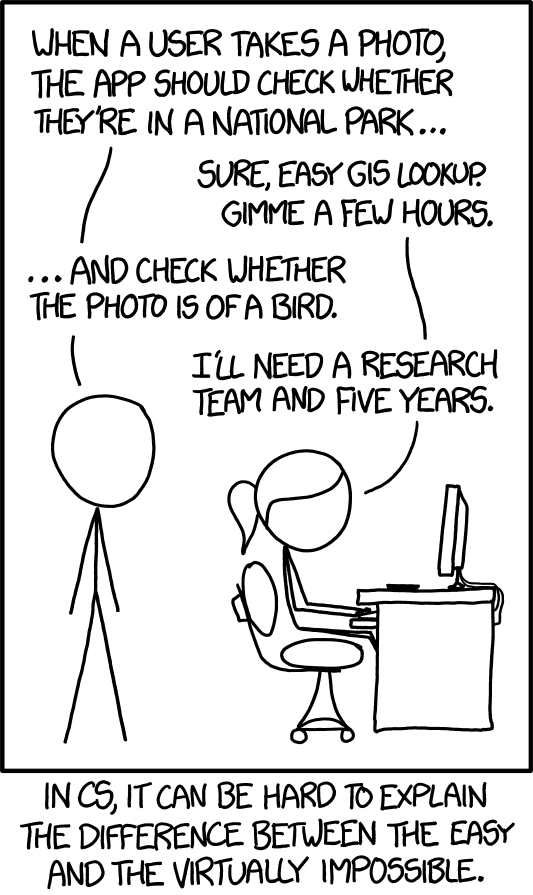
\includegraphics[height=4.5cm]{bird.png}}

\clearpage

\textbf{Pre-trained CNNs}

A convolutional neural network consists of 




\end{document}
